% !TEX program = xelatex
\documentclass[11pt]{article}
\usepackage{fontspec}
\usepackage{xeCJK}
\usepackage[margin=1in]{geometry}
\usepackage{amsmath}
\usepackage{amssymb}
\usepackage{amsthm}
\usepackage{graphicx}
\usepackage{tikz-cd}
\usepackage{multicol}
\usepackage{titling}
\usepackage{setspace}
\usepackage{float}
\usepackage{subcaption}
\usepackage{algorithm}
\usepackage{algpseudocode}
\newtheorem{theorem}{Theorem}
\newtheorem{lemma}{Lemma}

% Bigger & bolder title
\pretitle{\begin{center}\LARGE\bfseries}
\posttitle{\par\end{center}\vskip 0.5em}
\predate{\begin{center}}
\postdate{\end{center}}
\setlength{\droptitle}{-6em}

% Paragraph style (old)
% \setlength{\parindent}{0pt}
% \setlength{\parskip}{0.4\baselineskip}
% Paragraph style (new)
% \setlength{\parindent}{2em}
% \setlength{\parskip}{0pt}
% \setstretch{0.96}


\begin{document}

\title{Notes on Coding Theory}
\author{}
\date{}
\maketitle

\clearpage
\section{Binary Linear Block Codes}
A $(n,k)$ binary linear block code is a $k$-dimensional subspace of the $n$-dimensional vector space, where $n$ is the length of the codewords and $k$ is the length of the data bits. Let $\mathcal{C}$ be a $(n,k)$ binary linear block code with codewords $\{ \boldsymbol{c}_1, \cdots, \boldsymbol{c}_{M-1} \}$. $\mathcal{C}$ is a subspace of $\mathbb{F}_2^n$, i.e., it is closed under vector addition 
\[
\boldsymbol{c}_i, \boldsymbol{c}_j \in \mathcal{C} \implies \boldsymbol{c}_i + \boldsymbol{c}_j \in \mathcal{C}
\]
and scalar multiplication
\[
\boldsymbol{c} \in \mathcal{C} \implies 0 \cdot \boldsymbol{c} \in \mathcal{C} \text{ and } 1 \cdot \boldsymbol{c} \in \mathcal{C}
\]

Note that,
\begin{itemize}
  \item Since we want to add redundancy, $n > k$
  \item The rate $R$ of the code is $R = \frac{k}{n}$
  \item Assuming the codewords are distinct, the size of the code, i.e., the number of codewords, is $M = 2^k$.
\end{itemize}
To make a "good code", it is desired to have high rate, low probability of decoding error, and omputationally efficient to encode and decode.

\subsection{Generator matrix}
A $(n,k)$ linear block code (LBC) is defined  in terms of $k$ length-$n$ binary vectors, $(\boldsymbol{g_1}, \cdots, \boldsymbol{g_k})$. A sequence of $k$ data bits, $x = (x_1, \cdots , x_k)$ is mapped to a length-$n$ codeword $\boldsymbol{c}$ as follows,
\[
\boldsymbol{c} = x_1 \boldsymbol{g_1} + \cdots + x_k \boldsymbol{g_k}
\]
which can be expressed compactly as,
\[
\boldsymbol{c} = \boldsymbol{x} G, \quad \text{where} \quad G = \left[ \begin{matrix} \boldsymbol{g_1} \\ \boldsymbol{g_2} \\ \vdots \\ \boldsymbol{g_k} \end{matrix} \right]
\]
The $k \times n$ matrix $G$ is called a \textbf{generator matrix} of the code, $k$ is called the code dimension, $n$ is the block length. Assuming $\boldsymbol{c}$, $\boldsymbol{g}$ are row vectors.

Note that, the generator matrix for a code (i.e., a set of codewords) is not unique. We may have different generator matrix $G$ of same shape and yields same set of codewords, but with different mappings. Among all possible generator matrices for a code, we often prefer
one that is of the form
\[
G = \left[ I_k \mid  P \right]
\]
where $I_k$ is the $k \times k$ identity matrix and $P$ is a $k \times (n - k)$ matrix. Such a $G$ is called a \textbf{systematic generator matrix}. Thus,
\[
\boldsymbol{c} = \boldsymbol{x} G = \boldsymbol{x} \left[ I_k \mid  P \right] = \left[ \boldsymbol{x}  \mid  \boldsymbol{x} P \right]
\]
In a systematic code, the length-$n$ codeword consists of the $k$ data bits $\boldsymbol{x}$, followed by $(n - k)$ parity bits $\boldsymbol{x} P$.

Given any generator matrix, we can find a systematic version by elementary row operations: if $G_1$ is obtained from $G_2$ via elementary row operations, then
$G_1$, $G_2$ have the same set of codewords; only the mappings are different.

\subsection{Parity check matrix}

The orthogonal complement of $\mathcal{C}$, denoted $\mathcal{C}^\perp$ is defined as the set of all vectors in $\mathbb{F}_2^n$ that are orthogonal to each vector in $\mathcal{C}$. Therefore,
\begin{itemize}
  \item $\mathcal{C}^\perp$ is a subspace of $\mathbb{F}_2^n$, if $\boldsymbol{u} \text{,} \boldsymbol{v} \in \mathcal{C}^\perp$, then for any $\boldsymbol{c} \in \mathcal{C}$,
  \[
  \boldsymbol{c}\boldsymbol{u}^T = 0 \, \text{ and } \, \boldsymbol{c}\boldsymbol{v}^T = 0 \, \Rightarrow \, \boldsymbol{c}(\boldsymbol{u} + \boldsymbol{v})^T = 0 \, \Rightarrow \, (\boldsymbol{u} + \boldsymbol{v}) \in \mathcal{C}^\perp
  \]
  \item Since $\mathcal{C}$ has dimension $k$, $\mathcal{C}^\perp$ has dimension $(n - k)$ 
  \item Thus, the basis for $\mathcal{C}^\perp$ is $(\boldsymbol{h_1}, \cdots, \boldsymbol{h_{n-k}})$, which can be expressed compactly as a $(n-k) \times n$ matrix,
  \[
  H = \left[ \begin{matrix} \boldsymbol{h_1} \\ \boldsymbol{h_2} \\ \vdots \\ \boldsymbol{h_{n-k}} \end{matrix} \right]
  \]
  which is called the \textbf{parity check matrix}.
  \item Each codeword $\boldsymbol{c} \in \mathcal{C}$ is orthogonal to each row of $H$ (i.e. the binary dot-product of a codeword with each row of $H$ is $0$, $\boldsymbol{c} H^T = \boldsymbol{0}$)
  \item For a systematic generator matrix $G = \left[ I_k \mid  P \right]$
  \[
  \boldsymbol{c} H^T = \boldsymbol{0} \Rightarrow \boldsymbol{x} G H^T = \boldsymbol{0} \text{ for all } \boldsymbol{x} \Rightarrow G H^T = 0
  \]
  \[
  GH^T = \left[I_k \mid P\right] \begin{bmatrix} -P \\ I_{n-k} \end{bmatrix} = I_k (-P) + P I_{n-k} = -P + P = 0
  \]
  the systematic parity check matrix is given by $H = \left[ -P^T \mid  I_{n-k} \right]$.
\end{itemize}

\subsection{Minimum distance of a code}
The \textbf{Hamming distance} $d(\boldsymbol{x}, \boldsymbol{y})$ between two binary sequences $\boldsymbol{x}, \boldsymbol{y}$ of length $n$ is the number of positions in which $\boldsymbol{x}$ and $\boldsymbol{y}$ differ.

Let $\mathcal{C}$ be a code with codewords $\{ \boldsymbol{c}_1, \cdots, \boldsymbol{c}_{M} \}$. Then the
minimum distance $d_{\min}$ is the smallest Hamming distance
between any pair of codewords. That is,
\[
d_{\min} = \min_{i \neq j} d(\boldsymbol{c}_i, \boldsymbol{c}_j)
\]
also, the Hamming distance between two codewords $\boldsymbol{u}, \boldsymbol{v}$ can expressed as
\[
d(\boldsymbol{u}, \boldsymbol{v}) = wt(\boldsymbol{u} + \boldsymbol{v})
\]
where $wt(\boldsymbol{c})$ is the Hamming weight of $\boldsymbol{c}$, i.e., the number of nonzero elements in $\boldsymbol{c}$. Thus,
\[
\begin{aligned}
d_{\min} = \min_{i \neq j} d(\boldsymbol{c}_i, \boldsymbol{c}_j) &= \min_{i \neq j} wt(\boldsymbol{c}_i + \boldsymbol{c}_j) \\
&= \min_{\boldsymbol{c}_k \neq \boldsymbol{0}} wt(\boldsymbol{c}_k) \quad \text{(since $\boldsymbol{c}_i + \boldsymbol{c}_j$ is also a codeword)}
\end{aligned}
\]
the minimum distance of an LBC equals the minimum Hamming weight among the non-zero codewords.

Also, the minimum distance of an LBC code can be found by looking at its parity-check matrix $H$: the minimum distance $d_{\min}$ of the code $\mathcal{C}$ is
the minimum number of columns of $H$ that are linearly dependent, i.e., that can be combined to give the zero vector.

\subsection{Optimal decoding of a block code: ML decoding}
For any channel described by $P_{Y \mid X}$ , if the input bits/messages
corresponding to the codewords are equally likely, then the optimal
decoder given the received length-$n$ sequence $\boldsymbol{y}$ is the
maximum likelihood decoder given by
\[
\hat{\boldsymbol{x}} = \arg\max_{\boldsymbol{x} \in \mathcal{C}} P(\boldsymbol{y} \mid \boldsymbol{x})
\]

If the BSC probability $\epsilon < \frac{1}{2}$, then the codeword with smallest Hamming distance is the ML decoding
\[
\hat{\boldsymbol{x}} = \arg\min_{\boldsymbol{x} \in \mathcal{C}} d(\boldsymbol{y}, \boldsymbol{x})
\]

Draw spheres of radius $t$ centred on each codeword. Sphere centred at $\boldsymbol{c}_i$
contains all the binary sequences $\boldsymbol{r}$ such that $d(\boldsymbol{c}_i, \boldsymbol{r}) \leq t$.
\begin{figure}[H]
  \centering
  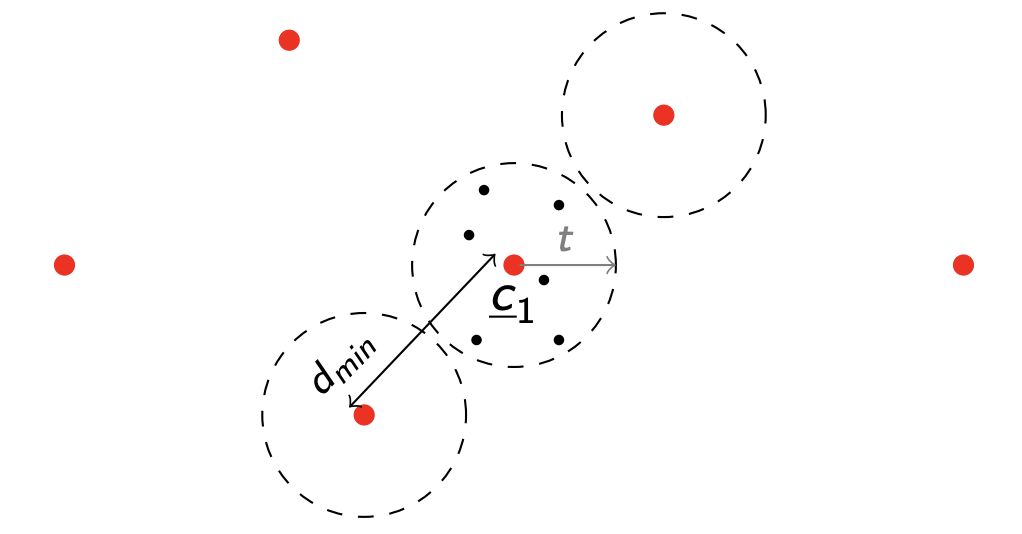
\includegraphics[width=0.5\linewidth]{images/mindis.png}
  \caption{The big dots represent the codewords, the little ones are the other length-$n$ binary sequences}
  \label{fig:ML-decoding}
\end{figure}
\noindent If fewer than $t$ errors occur, the received word $\boldsymbol{r}$ will lie within
the radius-$t$ sphere of the transmitted codeword. Further, the spheres won't overlap if $2t < d_{\min}$, or
$2t \leq d_{\min} - 1$.

Therefore, \textbf{a block code with minimum distance $d_{\min}$ is guaranteed to correct any pattern of up to $\mathbf{\left\lfloor \frac{d_{\min} - 1}{2} \right\rfloor}$ errors}. It can recover up to $d_{\min} - 1$ erasures.

$d_{\min}$ gives the guaranteed error correction capability of a code, but the code may be able to correct many more error patterns.

\subsection{Syndrome decoding}
For any received $n$ bits string $\boldsymbol{r}$, a \textbf{syndrome vector} can be calculated as
\[
H \boldsymbol{r}^\top = \boldsymbol{s}
\]
where, in the context of $GF(2)$,
$\boldsymbol{r} \in \mathbb{F}_2^{1 \times n}$, $\boldsymbol{s} \in \mathbb{F}_2^{1 \times (n-k)}$.

By writing the received $\boldsymbol{r}$ in the form of $\boldsymbol{r} = \boldsymbol{c} + \boldsymbol{e}$, where $\boldsymbol{c}$ is a codewords and $\boldsymbol{e}$ is the error pattern introduced in the channel. Therefore,
\[
H \boldsymbol{r}^\top = H (\boldsymbol{c} + \boldsymbol{e})^\top = H \boldsymbol{e}^\top = \boldsymbol{s}
\]
Thus, utilizing this property, we can precompute the syndromes for every possible error patterns and store them into a lookup table.
Then, for a received $\boldsymbol{r}'$ and its syndrome, we can find the corresponding error pattern $\boldsymbol{e}'$ from the lookup table, then, the decoding result is
\[
\boldsymbol{c}' = \boldsymbol{r}' - \boldsymbol{e}' = \boldsymbol{r}' + \boldsymbol{e}'
\]
where $+$ and $-$ are equivalent operation in $GF(2^q)$.


\clearpage
\section{Low-Density Parity-Check Codes}

Low-density parity-check (LDPC) codes are a class of linear block codes with implementable decoders, which provide near-capacity performance on a large set of data-transmission and data-storage channels.

\subsection{Representation of LDPC Codes}

A low-density parity-check code is a linear block code given by the null space of an $m \times n$ parity-check matrix \textbf{H} that has a low density of 1s. The density need only be sufficiently low to permit effective iterative decoding.

\[
    \mathbf{H} \in \{0,1\}^{m \times n}, \qquad \mathbf{H}\mathbf{t} = \mathbf{0} \quad \text{for all codewords } \mathbf{t}
\]

LDPC codes can be classified as:
\begin{itemize}
  \item A regular LDPC code is a linear block code whose parity-check matrix \textbf{H} has fixed column weight $g$ and row weight $r$, where $r/g = n/m$ and $g \ll m$. In this case, the code rate $R$ is bounded by $R \geq 1 - \frac{m}{n} = 1 - \frac{g}{r}$ with equality when \textbf{H} is full rank.
  \item An irregular LDPC code is a linear block code whose parity-check matrix \textbf{H} has variable column weights and row weights, being determined by code-design procedures.
\end{itemize}

\noindent Additionally, almost all LDPC code constructions impose the structural property on \textbf{H}: no two rows or two columns have more than one position in common that contains a nonzero element.

Graphically, \textbf{Tanner graphs} are used to represent a LDPC code from its parity-check matrix \textbf{H}. Tanner graph is a bipartite graph, that is, a graph whose nodes may be separated into two types, with edges connecting only nodes of different types. The two types of nodes in a Tanner graph are the variable nodes (or code-bit nodes) and the check nodes (or constraint nodes), which are denoted by VNs and CNs, respectively.

In a Tanner graph, CN i is connected to VN j whenever element $h_{ij}$ in \textbf{H} is a $1$. Therefore, there are m CNs in a Tanner graph, one for each check equation, and n VNs, one for each code bit; the m rows of \textbf{H} specify the m CN connections, and the n columns of \textbf{H} specify the n VN connections. This is the basis of \textbf{iterative decoding}: each of the nodes acts as a locally operating processor and each edge acts as a bus that conveys information from a given node to each of its neighbors.

\begin{figure}[H]
  \centering
  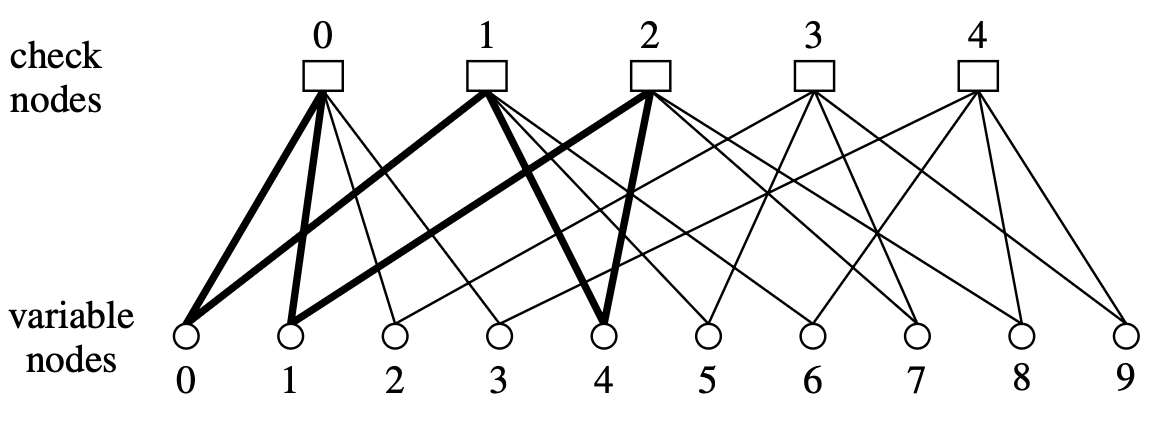
\includegraphics[width=0.5\linewidth]{images/Tannerdemo.png}
  \caption{Tanner graph of a (10,5) linear block code with $r = 4$, $g = 2$ (i.e. the degree of each VN is 2 and the degree of each CN is 4)}
  \label{fig:tanner-demo}
\end{figure}

The parity-check matrix for the Tanner graph above is 
\[
\mathbf{H} =
\begin{bmatrix}
1 & 1 & 1 & 1 & 0 & 0 & 0 & 0 & 0 & 0 \\
1 & 0 & 0 & 0 & 1 & 1 & 1 & 0 & 0 & 0 \\
0 & 1 & 0 & 0 & 1 & 0 & 0 & 1 & 1 & 0 \\
0 & 0 & 1 & 0 & 0 & 1 & 0 & 1 & 0 & 1 \\
0 & 0 & 0 & 1 & 0 & 0 & 1 & 0 & 1 & 1
\end{bmatrix}.
\]
As follows from $\mathbf{v}\mathbf{H}^{T} = \mathbf{0}$, that the bit values connected to the same check node must sum to zero (mod 2). Also, since rank(\textbf{H}) $= 4 \neq 5$, \textbf{H} is not full rank, so the code rate is $R = 1- 4/10 = 3/5$. As shown in \ref{fig:tanner-demo}, the six thickened edges form a \textbf{closed path}, which is called a \textbf{cycle}. The length of a cycle is equal to the number of edges which form the cycle: a cycle of length l is often called on l-cycle, and the minimum cycle length in a given bipartite graph is called the \textbf{graph's girth}.

It is possible to more closely approach capacity limits with irregular LDPC codes than with regular LDPC codes. For irregular LDPC codes, the parameters g and r vary with the columns and rows, so it is usual to specify the VN and CN \textbf{degree-distribution polynomials}. In the polynomial,
\[
\lambda(X) = \sum_{d=1}^{d_v} \lambda_d X^{d-1},
\]
$\lambda_d$ denotes the fraction of all edges connected to degree-$d$ VNs and $d_v$ denotes the maximum VN degree. Similarly, in the polynomial
\[
\rho(X) = \sum_{d=1}^{d_c} \rho_d X^{d-1},
\]
$\rho_d$ denotes the fraction of all edges connected to degree-$d$ CNs and $d_c$ denotes the maximum CN degree. Note that, for the regular code above, for which $g = 2$ and $r = 4$, we have $\lambda(X) = X$ and $\rho(X) = X^3$. It is also possible to view this from a node perpective, $L(X) = \sum_{d=1}^{d_v} L_d X^{d}$ and $R(X) = \sum_{d=1}^{d_c} R_d X^{d}$, where $L_d = \frac{\lambda_d/d}{\int_0^1 \lambda(X)\,dX}$ and $R_d = \frac{\rho_d/d}{\int_0^1 \rho(X)\,dX}$.

The average degrees are $\bar{d}_v = L'(1) = \left(\int_0^1 \lambda(x)\,dx\right)^{-1}$ and $\bar{d}_c = R'(1) = \left(\int_0^1 \rho(x)\,dx\right)^{-1}$. The design rate of an LDPC code is $R \geq 1 - \frac{\bar{d}_v}{\bar{d}_c} = 1 - \frac{L'(1)}{R'(1)} = 1 - \frac{\int_0^1 \rho(x)\,dx}{\int_0^1 \lambda(x)\,dx}$. 

\clearpage
\subsection{Message Passing and the Turbo Principle}

\textbf{Message-passing decoding} refers to a collection of low-complexity decoders working in a distributed fashion to decode a received codeword in a concatenated coding scheme.

\begin{figure}[H]
  \centering
  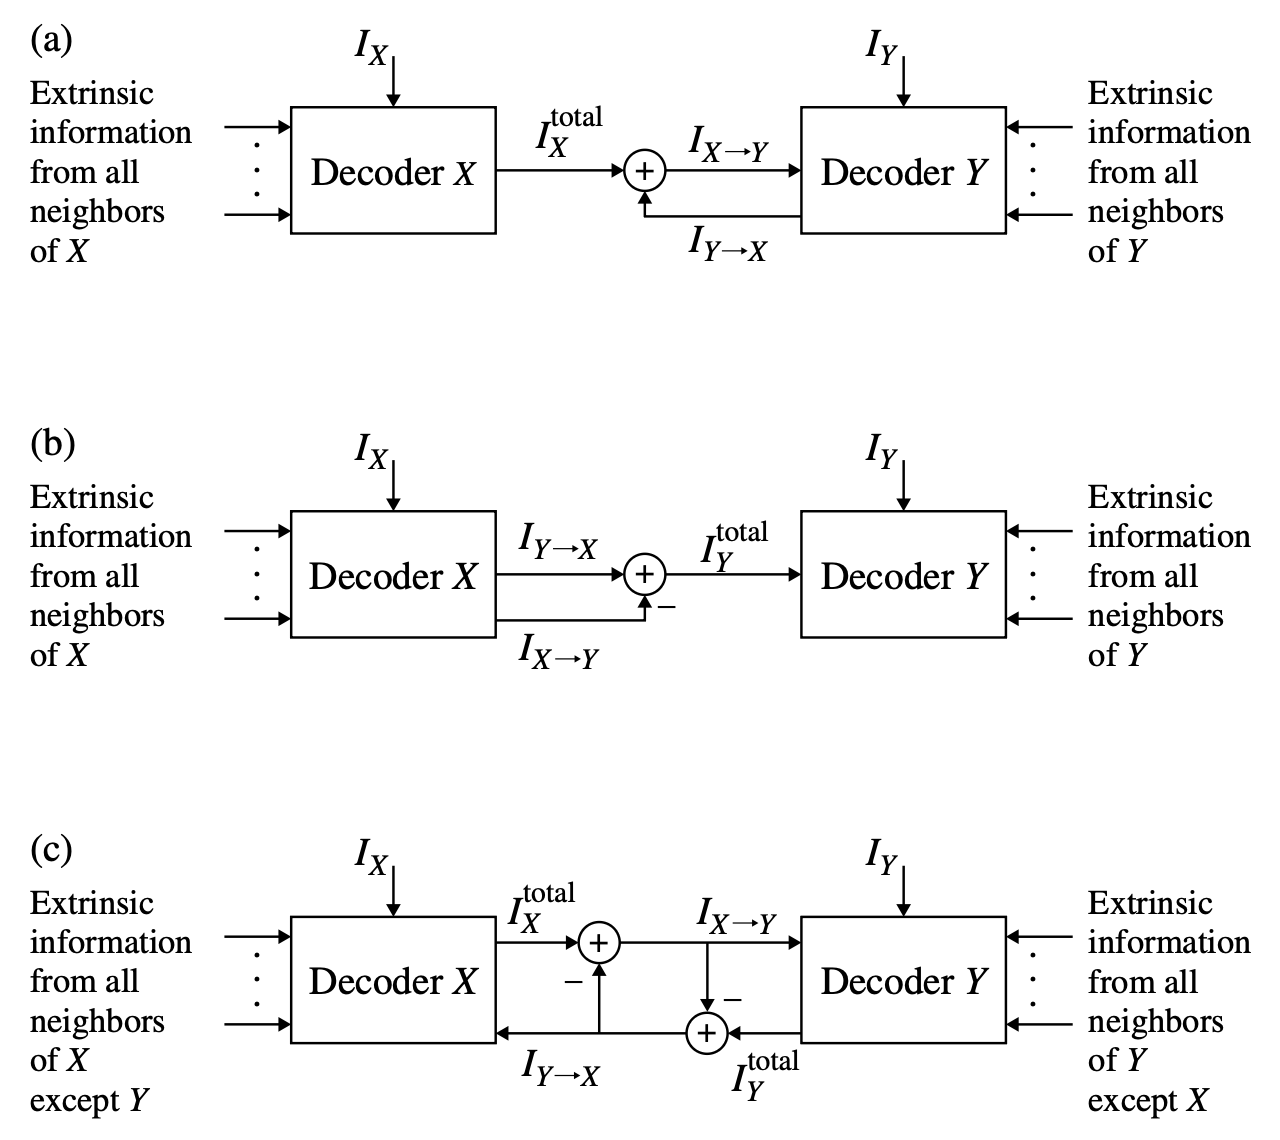
\includegraphics[width=0.5\linewidth]{images/turboprinciple.png}
  \caption{A depiction of the trubo principle for concatenated coding schemes.(a) Extrinsic information $I_{X \to Y}$ from decoder X to decoder Y. (b) Extrinsic information $I_{Y \to X}$ from decoder Y to decoder X. (c) A compact symmetric combination of (a) and (b).}
  \label{fig:turbo}
\end{figure}

The notion of \textbf{extrinsic-information passing} is called the turbo principle in the context of the iterative decoding of concatenated codes in communication channels. \textbf{Total information}

\[
I^{\text{total}}_X = \sum_{Z \in N(X)} I_{Z \to X}  + I_X
\]
and the \textbf{extrinsic information}
\[
I_{X \to Y} = \sum_{Z \in N(X) - \{Y\}} I_{Z \to X}  + I_X
\]
where $I_X$ denotes the \textbf{intrinisic information} received from the channel. Essentially, Y receives the sum total of messages that
X has available minus the information that Y already has, which means X does not pass to a neighboring decoder any information that the neighboring decoder already has.

\clearpage
\subsection{Sum-Prudct Algorithm}
The sum-product algorithm (SPA) or belief propagation algorithm (BPA) for general memoryless binary-input channels applies the turbo principle to correct the errors present in the received code bits.

In the context LDPC code, it can be considered as \textit{a generalized concatenation of many Single-Parity-Check code (CNs) and Repetition code (VNs)}, and they work cooperatively in a distributed fashion to determine the correct code bit values.

\begin{figure}[H]
  \centering
  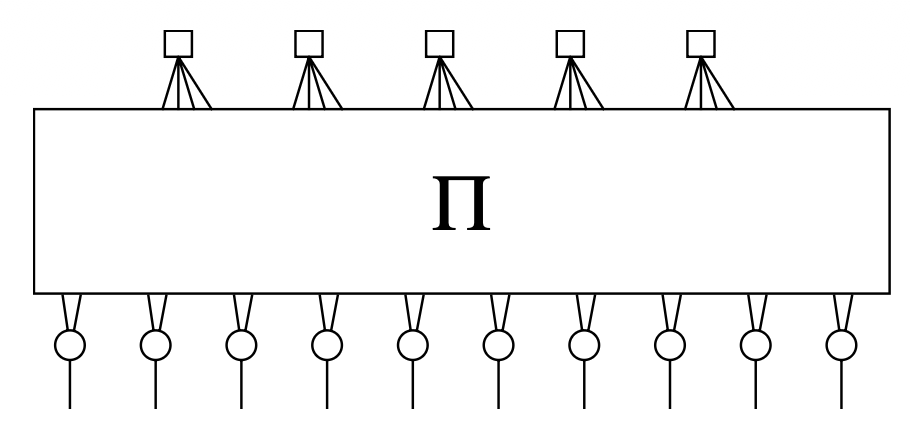
\includegraphics[width=0.5\linewidth]{images/LDPCgraph.png}
  \caption{Graphical representation of an LDPC code as a concatenation of SPC and REP codes. $\pi$ represents an interleaver.}
  \label{fig:LDPC-demo}
\end{figure}

The optimality criterion underlying the development of the SPA decoder is symbol-wise maximum a posteriori (MAP). we are interested in computing the a posteriori probability (APP) that a specific bit in the
transmitted codeword $\mathbf{v} = [v_0 \; v_1 \; \cdots \; v_{n-1}]$ equals to 1, given the received codeword $\mathbf{y} = [y_0 \; y_1 \; \cdots \; y_{n-1}]$. For a general code bit $v_j$, the APP is 
\[
\Pr(v_j = 1 \mid \mathbf{y})
\]
the APP ratio (or likelihood ratio under the uniform priors assumption),
\[
l(v_j \mid \mathbf{y}) \triangleq \frac{\Pr(v_j = 0 \mid \mathbf{y})}{\Pr(v_j = 1 \mid \mathbf{y})}
\]
or log-likelihood ratio (LLR) can be used for numerical stability,
\[
L(v_j \mid \mathbf{y}) \triangleq 
\log\left(\frac{\Pr(v_j = 0 \mid \mathbf{y})}{\Pr(v_j = 1 \mid \mathbf{y})}\right)
\]

The VN and CN decoders work cooperatively and iteratively to estimate $L(v_j \mid \mathbf{y})$ for $j = 0, 1, . . ., n-1$. Throughout our development, the \textbf{flooding schedule} is employed. According to this schedule, all VNs process their inputs and pass extrinsic information up to their neighboring check nodes; the check nodes then process their inputs and pass extrinsic information down to their neighboring variable nodes; and the procedure repeats, starting with the variable nodes. After a preset maximum number of iterations of this VN/CN decoding round, or after some stopping criterion has been met, the decoder computes (estimates) the LLRs $L(v_j \mid \mathbf{y})$ from which decisions on the bits $v_j$ are made. When the cycles are large, the estimates will be very accurate and the decoder will have near-optimal (MAP) performance. 

SPA assumes the \textit{LLR quantities received at each node from its neighbors are independent}. Clearly this breaks down when the \textit{number of iterations exceeds half of the Tanner graph's girth}.

\subsubsection{VN: Repetition Code MAP Decoder and APP Processor}

\begin{figure}[H]
  \centering
  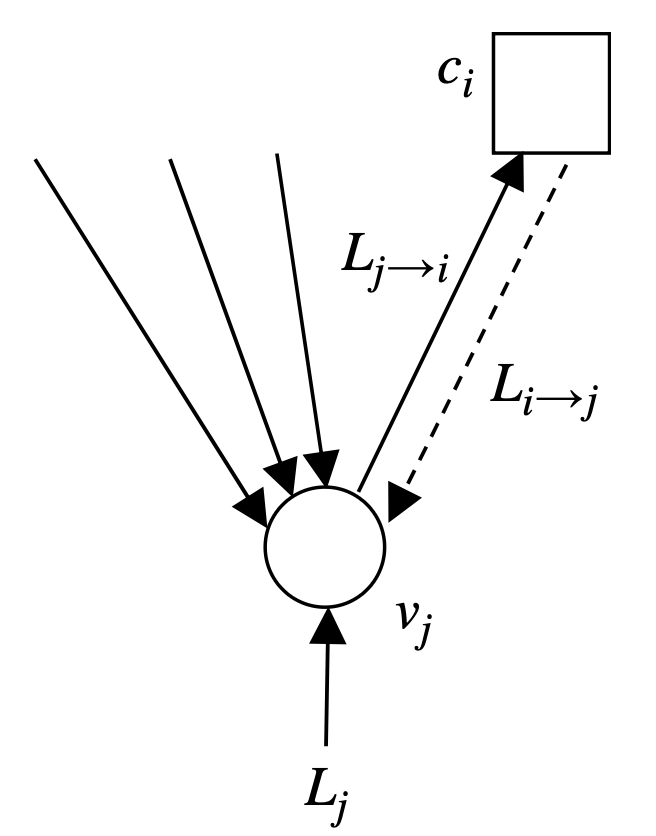
\includegraphics[width=0.5\linewidth]{images/VNpassing.png}
  \caption{A VN decoder (REP decoder). VN $j$ receives LLR information from the channel and from all of its neighbors, excluding message $L_{i \to j}$ from CN $i$, from which VN $j$ composes message $L_{j \to i}$ that is sent to CN $i$}
  \label{fig:VN-demo}
\end{figure}

Consider a REP code in which the binary code symbol $c \in \{0,1\}$ is transmitted over a memoryless channel $d$ times so that the $d$-vector $\mathbf{r}$ is received. By definition, the MAP decoder computes the log-APP ratio
\[
L(c \mid \mathbf{r}) = \log\left(\frac{\Pr(c = 0 \mid \mathbf{r})}{\Pr(c = 1 \mid \mathbf{r})}\right) = \log\left(\frac{\Pr(\mathbf{r} \mid c = 0)}{\Pr(\mathbf{r} \mid c = 1)}\right)
\]
under an equally likely assumption for the value of $c$ (ratio of a posterior = ratio of likelihood)

This simplifies as
\[
\begin{aligned}
L(c \mid \mathbf{r})
&= \log\left(\frac{\prod_{l=0}^{d-1} \Pr(r_l \mid c = 0)}{\prod_{l=0}^{d-1} \Pr(r_l \mid c = 1)}\right) \\
&= \sum_{l=0}^{d-1} \log\left(\frac{\Pr(r_l \mid c = 0)}{\Pr(r_l \mid c = 1)}\right) = \sum_{l=0}^{d-1} L(r_l \mid x)
\end{aligned}
\]
where $L(r_l \mid x)$ is obviously defined. Thus, the MAP receiver for a REP code computes the LLRs for each channel output $r_l$ and adds them. \textit{The MAP decision is $\hat{c} = 0$ if $L(c \mid \mathbf{r}) \geq 0$ and $\hat{c} = 1$ otherwise.}

In the context of LDPC decoding, the above expression is adapted to compute the extrinsic information to be sent from VN $j$ to CN $i$ of Figure~\ref{fig:VN-demo},
\[
\boxed{
L_{j \to i} = L_j + \sum_{i' \in N(j) - \{i\}} L_{i' \to j}
}
\]
The quantity $L_j$ in this expression is the LLR value computed from the channel sample $y_j$,
\[
L_j = L(c_j \mid y_j) = \log\left(\frac{\Pr(c_j = 0 \mid y_j)}{\Pr(c_j = 1 \mid y_j)}\right).
\]
At the last iteration, VN $j$ produces a decision based on
\[
L_j^{\text{total}} = L_j + \sum_{i \in N(j)} L_{i \to j}
\]

\subsubsection{CN: Single-Parity-Check Code MAP Decoder and APP Processor}

\begin{figure}[H]
  \centering
  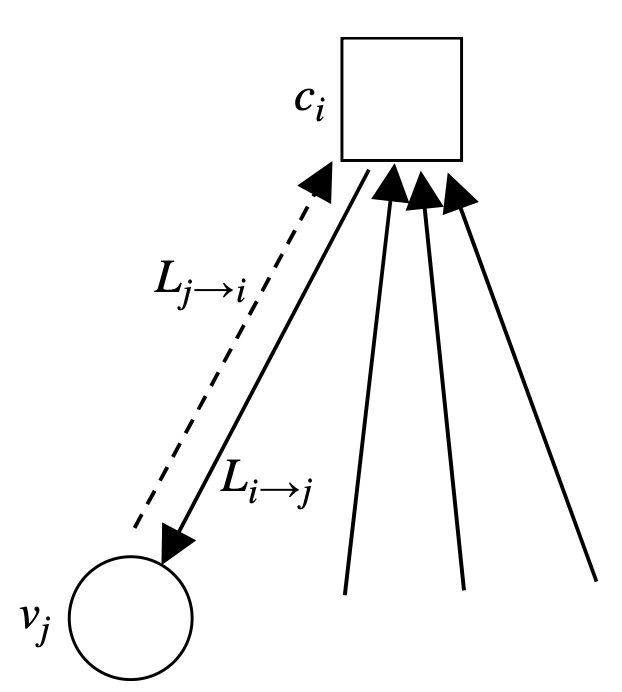
\includegraphics[width=0.5\linewidth]{images/CNpassing.png}
  \caption{A CN decoder (SPC decoder). CN $i$ receives LLR information from all of its neighbors, excluding message $L_{j \to i}$ from VN $j$, from which CN $i$ composes message $L_{i \to j}$ that is sent to VN $j$}
  \label{fig:CN-demo}
\end{figure}

\begin{lemma}
\label{lem:gallager-even-odd}
  Consider a vector of $d$ independent binary random variables $\mathbf{a} = [a_0, a_1, \ldots, a_{d-1}]$ in which $\Pr(a_l = 1) = p_1^{(l)}$ and $\Pr(a_l = 0) = p_0^{(l)}$. Then the probability that $\mathbf{a}$ contains an even number of 1s is
\[
\frac{1}{2} + \frac{1}{2}\prod_{l=0}^{d-1}\left(1 - 2p_1^{(l)}\right),
\]
and the probability that $\mathbf{a}$ contains an odd number of 1s is
\[
\frac{1}{2} - \frac{1}{2}\prod_{l=0}^{d-1}\left(1 - 2p_1^{(l)}\right).
\]
\end{lemma}

Consider the transmission of a length-$d$ SPC codeword $\mathbf{c}$ over a memoryless channel whose output is $\mathbf{r}$. The bits in the codeword $\mathbf{c}$ have a single constraint: \textit{there must be an even number of 1s in $\mathbf{c}$}. Without loss of generality, we focus on bit $c_0$, for which the MAP decision rule is
\[
\hat{c}_0 = \arg\max_{b \in \{0,1\}} \Pr(c_0 = b \mid \mathbf{r}, \mathrm{SPC}),
\]
where the conditioning on SPC is a reminder that there is an SPC constraint imposed on $\mathbf{c}$. Consider now
\[
\begin{aligned}
\Pr(c_0 = 0 \mid \mathbf{r}, \mathrm{SPC})
&= \Pr(c_1, c_2, \ldots, c_{d-1} \text{ has an even number of 1s} \mid \mathbf{r}) \\
&= \frac{1}{2} + \frac{1}{2}\prod_{l=1}^{d-1}\left(1 - 2\Pr(c_l = 1 \mid r_l)\right),
\end{aligned}
\]
where the second line follows from the \ref{lem:gallager-even-odd}. Rearranging gives
\[
1 - 2\Pr(c_0 = 1 \mid \mathbf{r}, \mathrm{SPC}) = \prod_{l=1}^{d-1}\left(1 - 2\Pr(c_l = 1 \mid r_l)\right),
\]
where $p(c_0 = 0 \mid \mathbf{r}, \mathrm{SPC}) = 1 - p(c_0 = 1 \mid \mathbf{r}, \mathrm{SPC})$. 

We can change this to an \textbf{LLR representation} using the easily proven relation for a generic binary random variable with probabilities $p_1$ and $p_0$,
\[
1 - 2p_1 = \tanh\left(\frac{1}{2}\log\left(\frac{p_0}{p_1}\right)\right) = \tanh\left(\frac{1}{2}\mathrm{LLR}\right).
\]
where here $\mathrm{LLR} = \log(p_0/p_1)$. Applying this relation gives
\[
\tanh\left(\frac{1}{2}L(c_0 \mid \mathbf{r}, \mathrm{SPC})\right)
= \prod_{l=1}^{d-1}\tanh\left(\frac{1}{2}L(c_l \mid r_l)\right)
\]
or
\[
L(c_0 \mid \mathbf{r}, \mathrm{SPC})
= 2\tanh^{-1}\left(\prod_{l=1}^{d-1}\tanh\left(\frac{1}{2}L(c_l \mid r_l)\right)\right).
\]
Thus, \textit{the MAP decoder for bit $c_0$ in a length-$d$ SPC code makes the decision $\hat{c}_0 = 0$ if $L(c_0 \mid \mathbf{r}, \mathrm{SPC}) \geq 0$ and $\hat{c}_0 = 1$ otherwise.}

In the context of LDPC decoding, when the CNs function as APP processors instead of MAP decoders, CN $i$ computes the extrinsic information
\[
\boxed{
L_{i \to j} = 2\tanh^{-1}\left(\prod_{j' \in N(i)-\{j\}} \tanh\left(\frac{1}{2}L_{j' \to i}\right)\right)
}
\]
and transmits it to VN $j$. 
\subsubsection{CN update equation generalized}
The CN update equation can also be written in the form of "sum" as in the VN updates,
\[
\boxed{
L_{i \to j} = \boxplus_{j' \in N(i) - {j}} \left\{ L_{j' \to i} \right\}
}
\]
where the boxplus operation $\boxplus$ is defined as
\[
x \boxplus y = \max^* (0, x+y) - \max^*(x,y) \quad \text{where} \quad \max^*(x,y) = \ln (e^x + e^y)
\]
In GF(2), the special case can be shown to be $x \boxplus y = 2\tanh^{-1}(\tanh(x/2) \tanh(y/2))$.


\subsubsection{The Gallager SPA Decoder}

\begin{algorithm}[H]
\caption{The Gallager Sum-Product Algorithm}
\begin{algorithmic}[1]
\State \textbf{Initialization:} For all $j$, initialize $L_j$ according to the appropriate channel model. Then, for all $i,j$ for which $h_{ij} = 1$, set $L_{j \to i} = L_j$.
\State \textbf{CN update:} Compute outgoing CN messages $L_{i \to j}$ for each CN using
  \[
  \begin{aligned}
  L_{i \to j} &= 2\tanh^{-1}\left(\prod_{j' \in N(i)-\{j\}} \tanh\left(\frac{1}{2}L_{j' \to i}\right)\right) \\
  &= \prod_{j' \in N(i)-\{j\}} \alpha_{j'i} \cdot \phi\left( \sum_{j' \in (i)-\{j\}} \phi(\beta_{j'i}) \right) \\
  & \text{where}\quad \phi(x) =-\log [\tanh (x/2)] = \log(\frac{e^x + 1}{e^x - 1}),\quad \alpha_{ji} = \text{sign}(L_{j \to i}),\quad \beta_{ji} = \mid L_{j \to i} \mid
  \end{aligned}
  \]
  and then transmit them to the VNs. Note that $\phi (x) = \phi ^ {-1}(x)$ for $x > 0$, which is less challenging to compute compare with the product of the $\tanh$ and $\tanh^{-1}$ functions.
\State \textbf{VN update:} Compute outgoing VN messages $L_{j \to i}$ for each VN using
  \[
  L_{j \to i} = L_j + \sum_{i' \in N(j)-\{i\}} L_{i' \to j},
  \]
  and then transmit them to the CNs.
\State \textbf{LLR total:} For $j = 0,1,\ldots,n-1$, compute
  \[
  L_j^{\text{total}} = L_j + \sum_{i \in N(j)} L_{i \to j}.
  \]
\State \textbf{Stopping criteria:} For $j = 0,1,\ldots,n-1$, set
  \[
  \hat{v}_j =
  \begin{cases}
  1, & \text{if } L_j^{\text{total}} < 0, \\
  0, & \text{otherwise,}
  \end{cases}
  \]
  to obtain $\hat{\mathbf{v}}$. If $\hat{\mathbf{v}}\mathbf{H}^{T} = \mathbf{0}$ or the number of iterations equals the maximum limit, stop; otherwise, go to Step 2.
\end{algorithmic}
\end{algorithm}

The decoder is initialized by setting all VN messages $L_{j \to i}$ equal to
\[
L_j = L(v_j \mid y_j) = \log\left(\frac{\Pr(v_j = 0 \mid y_j)}{\Pr(v_j = 1 \mid y_j)}\right),
\]
for all $j,i$ for which $h_{ij} = 1$. Here, $y_j$ represents the channel value that was actually received, that is, it is not a variable here. We consider the following special cases.

\textbf{BEC.} In this case, $y_j \in \{0,1,e\}$ and we define $p = \Pr(y_j = e \mid v_j = b)$ to be the erasure probability, where $b \in \{0,1\}$. Then it is easy to see that
\[
\Pr(v_j = b \mid y_j) =
\begin{cases}
1, & \text{when } y_j = b, \\
0, & \text{when } y_j = b^c, \\
1/2, & \text{when } y_j = e,
\end{cases}
\]
where $b^c$ represents the complement of $b$. From this, it follows that
\[
L(v_j \mid y_j) =
\begin{cases}
+\infty, & y_j = 0, \\
-\infty, & y_j = 1, \\
0, & y_j = e.
\end{cases}
\]

\textbf{BSC.} In this case, $y_j \in \{0,1\}$ and we define $\varepsilon = \Pr(y_j = b^c \mid v_j = b)$ to be the error probability. Then it is obvious that
\[
\Pr(v_j = b \mid y_j) =
\begin{cases}
1-\varepsilon, & \text{when } y_j = b, \\
\varepsilon, & \text{when } y_j = b^c.
\end{cases}
\]
From this, we have
\[
L(v_j \mid y_j) = (-1)^{y_j}\log\left(\frac{1-\varepsilon}{\varepsilon}\right).
\]
Note that knowledge of $\varepsilon$ is necessary.

\textbf{BI-AWGNC.} We first let $x_j = (-1)^{v_j}$ be the $j$th transmitted binary value; note that $x_j = +1(-1)$ when $v_j = 0(1)$. We shall use $x_j$ and $v_j$ interchangeably hereafter. The $j$th received sample is $y_j = x_j + n_j$, where the $n_j$ are independent and normally distributed as $\mathcal{N}(0,\sigma^2)$. Then it is easy to show that
\[
\Pr(x_j = x \mid y_j) = \left[1 + \exp\left(-2y_jx/\sigma^2\right)\right]^{-1},
\]
where $x \in \{\pm 1\}$ and, from this, that
\[
L(v_j \mid y_j) = 2y_j/\sigma^2.
\]
In practice, an estimate of $\sigma^2$ is necessary.

\textbf{Rayleigh.} Assuming an independent Rayleigh fading channel and the decoder has perfect channel state information. The model is similar to that of the AWGNC: $y_j= \alpha_j x_j + n_j$, where $\{ \alpha_j \}$ are independent Rayleigh random variables with unity variance. The channel transition probability in this case is
\[
\Pr(x_j = x \mid y_j) = \left[1 + \exp\left(-2\alpha_j y_j x/\sigma^2\right)\right]^{-1}.
\]
Then the variable nodes are initialized by
\[
L(v_j \mid y_j) = 2\alpha_j y_j/\sigma^2.
\]
In practice, estimates of $\alpha_j$ and $\sigma^2$ are necessary.

\subsubsection{The Min-Sum Decoder}
\begin{figure}[H]
  \centering
  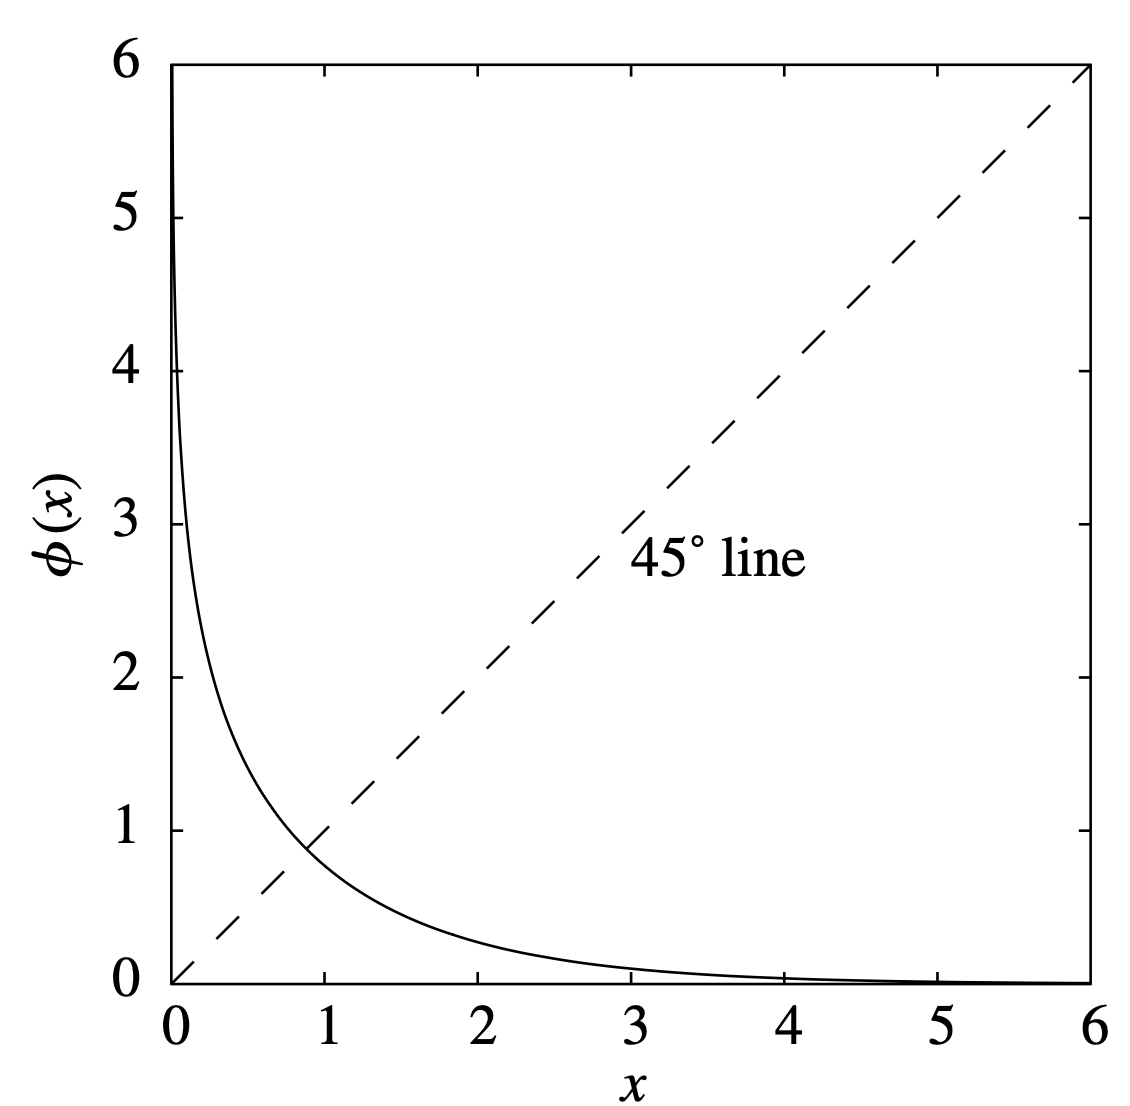
\includegraphics[width=0.5\linewidth]{images/phiplot.png}
  \caption{A plot of $\phi(x)$}
  \label{fig:phi}
\end{figure}

Consider the CN update equation in the Gallager SPA, from the shape of $\phi(x)$ that the largest term in the sum corresponds to the smallest $\beta_{ji}$ so that, assuming that this term dominates the sum,
\[
\phi\left(\sum_{j'} \phi(\beta_{j'i})\right)
\simeq
\phi\left(\phi\left(\min_{j'} \beta_{j'i}\right)\right)
=
\min_{j' \in N(i)-\{j\}} \beta_{j'i}
\]
Thus, the min-sum algorithm is simplt the log-domain SPA with Step 2 replaces by
\[
\text{CN update: } L_{i \to j}
=
\prod_{j' \in N(i)-\{j\}} \alpha_{j'i}
\cdot
\min_{j' \in N(i)-\{j\}} \beta_{j'i}.
\]
Note the fact that \textit{the sign of LLR represents the estimated code bit value (0 or 1) and the magnitude of LLR represents the confidence or reliability level of that estimate}. Therefore, the min-sum algorithm says that the CNs are only as confident as the least confident input.

\begin{figure}[H]
  \centering
  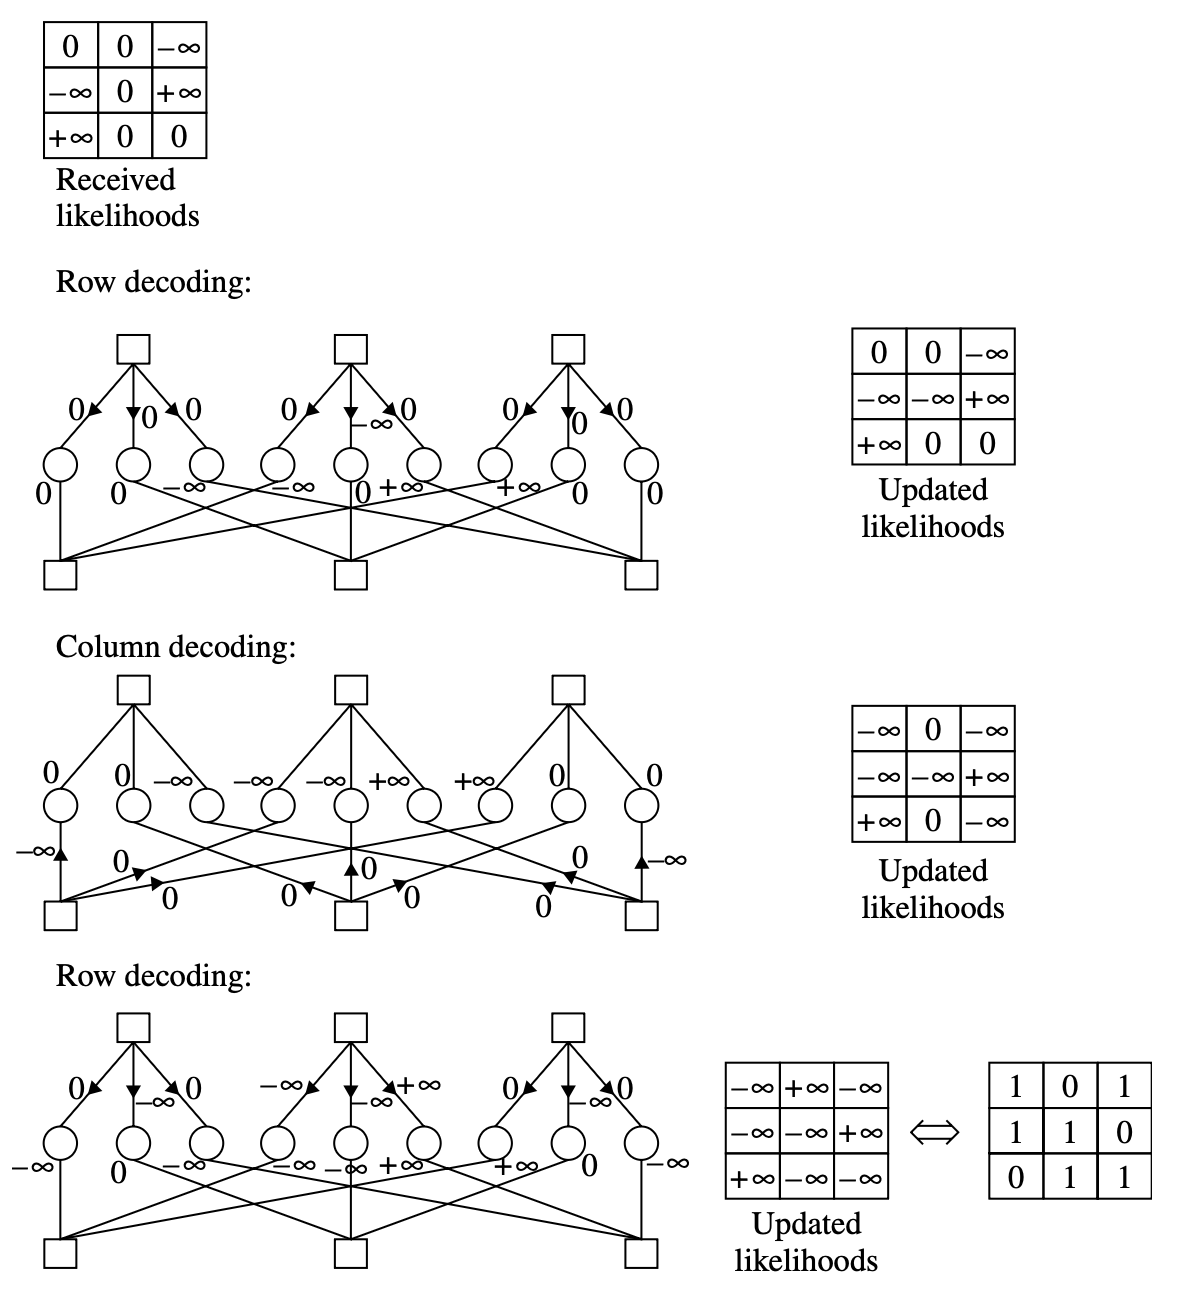
\includegraphics[width=0.5\linewidth]{images/minsumexample.png}
  \caption{An example of min-sum decoding on the BEC using the (3,2) regular LDPC code. Note that,for BEC, $\phi\left(\sum_{j'} \phi(\beta_{j'i})\right)$ is 0 or $\infty$ exactly when $min_{j'} \beta_{j'i}$ is 0 or $\infty$, respectively. Note also that this is equivalent to the iterative erasure filling algorithm.}
\end{figure}

Experimentally, for the first iteration of a min-sum decoder, the extrinsic information passed from a CN to a VN for a min-sum decoder is on average larger in magnitude than the extrinsic information that would have been passed by an SPA decoder. That is, the min-sum decoder is generally too optimistic in assigning reliabilities. Thus, we can use 
\[
\text{CN update: } L_{i \to j}
=
\prod_{j' \in N(i)-\{j\}} \alpha_{j'i}
\cdot c_{atten} \cdot
\min_{j' \in N(i)-\{j\}} \beta_{j'i}.
\]
where $0 < c_{atten} < 1$ is the arrenuation factor, usually $c_{atten} = 0.5$.

An alternative technique for mitigating the overly optimistic extrinsic information that occurs in a min-sum decoder is to subtract a constant offset $c_{offset} > 0$ from each CN-to-VN message magnitude $|L_{i \to j}|$, subject to the constraint that the result is non-negative. Thus, the offset-min-sum algorithm computes
\[
\text{CN update: } L_{i \to j}
=
\prod_{j' \in N(i)-\{j\}} \alpha_{j'i}
\cdot
\max\left\{
\min_{j' \in N(i)-\{j\}} \beta_{j'i} - c_{offset},\ 0
\right\}.
\]

\subsection{Decoding Algoithms for the BEC and the BSC}

The BEC and BSC are studied as special cases of the general SPA because their discrete channel outputs simplify the message-passing framework to simple symbolic operations. In the general SPA for the AWGN channel, received samples $y_j \in \mathbb{R}$ produce continuously-valued LLRs, and all Tanner graph messages are real-valued, requiring full nonlinear tanh-based computations at each node.

On the \textbf{BEC}, the LLR takes only three values $\{-\infty, 0, +\infty\}$, and the SPA reduces to iterative erasure filling --- a check node resolves an erasure only if exactly one neighbor is erased, collapsing the check node update to a simple XOR. Decoding failure is governed entirely by \textbf{stopping sets}, which cause failure even under ML decoding and are therefore a fundamental limitation of the code itself.

On the \textbf{BSC}, every received bit carries the same fixed-magnitude LLR $\log\frac{1-\varepsilon}{\varepsilon}$, providing no graded soft information. Gallager's \textbf{Algorithm A and B} exploit this by discarding soft information entirely, passing only binary hard decisions with XOR-based check node updates, achieving very low complexity at the cost of performance relative to full SPA.


\subsubsection{Iterative Erasure Filling for the BEC}
The iterative decoding algorithm for the BEC simply works to fill in the erased bits in such a way that all of the check equations contained in \textbf{H} are eventually satisfied.

\begin{algorithm}[H]
\caption{Iterative Erasure Decoding Algorithm}
\begin{algorithmic}[1]
\State Find all check equations (rows of \textbf{H}) involving a single erasure and solve for the values of bits corresponding to these erasures.
\State Repeat Step 1 until there exist no more erasures or until all equations are unsolvable.
\end{algorithmic}
\end{algorithm}

If no parity-check equation that involves only one of the erasures in the erasure set can be found, then none of the equations will be solvable and decoding will stop. Code bit sets that lead to unsolvable equations when they are erased are called \textbf{stopping sets}. Thus, a subset $S$ of code bits forms a stopping set if each equation that involves the bits in $S$ involves two or more of them. In Tanner graph, $S$ is a stopping set if all of its neighbors are connected to S at least twice. Such a configuration is problematic for an iterative decoder because, if these bits are erased, all equations involved will contain at least two erasures.

\subsubsection{ML Decoder for the BEC}
Adapted-\textbf{H} algorithm provides an example in which the stopping set
in the previous example is resolvable.

Suppose codeword $\mathbf{c}$ is transmitted over a BEC and the received word 
$\mathbf{r}$ has elements in $\{0, 1, e\}$. Let $J$ denote the index set of 
unerased positions and $J'$ the index set of erased positions. On the BEC, the ML criterion simplifies dramatically. The ML decoder selects the codeword $\hat{\mathbf{c}} \in \mathcal{C}$ maximising $P(\mathbf{r} \mid \mathbf{c})$, but since any codeword disagreeing with a received unerased bit has zero probability, ML reduces to finding the \textit{unique codeword consistent with all unerased positions}: 
\[
c_j = r_j \quad \forall\, j \in J
\]
Combined with the codeword validity constraint $\mathbf{c}\mathbf{H}^T = \mathbf{c}_{J'}\mathbf{H}_{J'}^T + \mathbf{c}_J \mathbf{H}_J^T = \mathbf{0}$, the ML criterion is fully expressed by the linear system:

\[
    \mathbf{c}_{J'}\mathbf{H}_{J'}^T = \mathbf{c}_J\mathbf{H}_J^T
\]
The right-hand side is fully known from the received word, so this is a linear 
system over $\text{GF}(2)$ in the unknown $\mathbf{c}_{J'}$. A unique solution 
exists if and only if the rows of $\mathbf{H}_{J'}^T$ are linearly independent, 
which requires $|J'| \leq n - k$. Since any $d_{\min} - 1$ rows of $\mathbf{H}^T$ 
are linearly independent, uniqueness is guaranteed whenever $|J'| < d_{\min}$.

To solve the linear system $\mathbf{c}_{J'}\mathbf{H}_{J'}^T = \mathbf{c}_J\mathbf{H}_J^T$ 
for the unknown erased bits $\mathbf{c}_{J'}$, apply Gaussian elimination to 
$\mathbf{H}$ targeting the erased columns $J'$, producing a modified matrix:

\[
    \tilde{\mathbf{H}} = \begin{bmatrix} \tilde{\mathbf{H}}_J & \tilde{\mathbf{H}}_{J'} \end{bmatrix}
\]
where $\tilde{\mathbf{H}}_J$ is the submatrix of $\tilde{\mathbf{H}}$ corresponding 
to the unerased columns $J$ modified by the elimination, and 
$\tilde{\mathbf{H}}_{J'}$ is the submatrix of $\tilde{\mathbf{H}}$ corresponding 
to the erased columns $J'$, which after elimination takes the form:

\[
    \tilde{\mathbf{H}}_{J'} = \begin{bmatrix} \mathbf{T} \\ \mathbf{M} \end{bmatrix}
\]
where $\mathbf{T}$ is a $|J'| \times |J'|$ lower-triangular matrix with ones on 
the diagonal, and $\mathbf{M}$ is an arbitrary binary matrix (which may be empty). 
The unknown erased bits $\mathbf{c}_{J'}$ are then recovered one at a time by 
back-substitution through the top $|J'|$ parity-check equations corresponding to 
$\mathbf{T}$, with the right-hand side fully computable from the known received 
bits $\mathbf{c}_J = \mathbf{r}_J$.

The system then becomes:
\[
    \mathbf{c}_{J'}\mathbf{T}^T = \mathbf{c}_J \tilde{\mathbf{H}}_J^T
\]
Since $\mathbf{T}$ is lower-triangular with ones on the diagonal, the unknown 
erased bits $\mathbf{c}_{J'}$ are recovered one at a time by back-substitution 
through the parity-check equations of $\tilde{\mathbf{H}}$. 

Thus, ML decoding on the BEC reduces entirely to Gaussian elimination over 
$\text{GF}(2)$ --- a linear algebraic operation with no probabilistic search 
required.


\subsubsection{Gallager's Algorithm A and B for the BSC}
As LLRs are trivial in BSC model, we use $M_{j \to i}$ and $M_{i \to j}$ to denote the LLR messages being passed $L_{j \to i}$ and $L_{j \to i}$.

Check node update equation for both algorithm A and B is
\[
M_{i \to j} =
\bigoplus_{j' \in N(i)-\{j\}} M_{j' \to i}
\]

For algorithm A, the variable node update equation is
\[
M_{j \to i}
=
\begin{cases}
M_j, & \text{if } \exists\, i' \in N(j)-\{i\} \text{ s.t. } M_{i' \to j} = M_j,\\
M_j^c, & \text{otherwise.}
\end{cases}
\]
where the outgoing message $M_{j \to i}$ is set to $M_j$ unless all of the
incoming extrinsic messages $M_{i'→j}$ disagree.

For algorithm A, the variable node update equation is
\[
M_{j \to i}
=
\begin{cases}
M_j^c, & \text{if } \left|\left\{ i' \in N(j)-\{i\} : M_{i' \to j} = M_j^c \right\}\right| \geq t,\\
M_j, & \text{otherwise.}
\end{cases}
\]
which means as long as there are more than $t$ incoming extrinsic information disagree with $M_j$ then the outgoing $M_{j \to i}$ is set to $M_j^c$

The code bit decisions for these algorithms are majority-based, as follows. If the degree of a variable node is odd, then the decision is set to the majority of the incoming check node messages. If the degree of a variable node is even, then the decision is set to majority of the check node messages and the channel message.

\subsubsection{The Bit-Flipping Algorithm for the BSC}
Noting that \textit{failed parity-check equations} are indicated by the elements of the syndrome, $\mathbf{s = r H^T}$, and that the \textit{number of failed parity checks for each code bit} is contained in the n-vector $\mathbf{f= sH}$ (operations over the integers). If the size of \textbf{H} is $m \times n$, then the size of \textbf{r, s, f} is $ 1 \times n$, $1 \times m$, $1 \times n$ respectively.

\begin{algorithm}[H]
\caption{The Bit-Flipping Algorithm}
\begin{algorithmic}[1]
\State Compute $\mathbf{s} = \mathbf{r}\mathbf{H}^{T}$ (operations over $\mathbb{F}^2$). If $\mathbf{s} = \mathbf{0}$, stop, since $\mathbf{r}$ is a codeword.
\State Compute $\mathbf{f} = \mathbf{s}\mathbf{H}$ (operations over $\mathbb{Z}$).
\State Identify the elements of $\mathbf{f}$ greater than some preset threshold, and then flip all the bits in $\mathbf{r}$ corresponding to those elements.
\State If the maximum number of iterations has not been reached, go to Step 1 using the updated $\mathbf{r}$.
\end{algorithmic}
\end{algorithm}


\clearpage
\subsection{Generalized LDPC Codes}
In a standard LDPC code, the two types of nodes in the Tanner graph perform 
simple operations. \textbf{Variable nodes (VN)} act as \textbf{repetition (REP) 
codes}, repeating the same bit value across all connected edges --- a degree-$d_v$ 
variable node is equivalent to a rate-$1/d_v$ repetition code. \textbf{Check nodes 
(CN)} act as \textbf{single parity-check (SPC) codes}, enforcing that the XOR of 
all connected bits equals zero. A standard LDPC code can therefore be viewed as a 
graph-based concatenation of REP and SPC component codes.

A \textbf{Generalized LDPC (GLDPC)} code replaces these simple component codes with 
stronger linear block codes. Check nodes are replaced by arbitrary linear block codes 
(e.g.\ Hamming, BCH, or Reed--Solomon codes) that enforce richer constraints than a 
single parity check, while variable nodes may similarly be replaced by stronger codes 
beyond simple repetition. The belief propagation (BP) decoder naturally extends to 
GLDPC codes: the simple REP and SPC message-passing rules at each node are replaced 
by the \textbf{a posteriori probability (APP) processor} for the corresponding 
component code, while the overall graph structure and message-passing framework remain unchanged.

The primary advantage of GLDPC codes is improved \textbf{minimum distance} for finite 
block lengths, which directly reduces the error floor, along with faster convergence 
due to stronger per-iteration information exchange. The cost is increased decoding 
complexity per node, since each check node now runs a full sub-decoder rather than a 
simple XOR operation.

\clearpage
\subsection{Code Ensemble Behaviour}

A \textbf{LDPC code ensemble $\mathcal{C}(n, \lambda, \rho)$} is a probability distribution over a set of LDPC codes sharing the same block length $n$, variable node degree distribution $\lambda(x)$, and check node degree distribution $\rho(x)$. A specific code is drawn from the ensemble by constructing a random Tanner graph via a uniformly random matching between variable node and check node edge sockets consistent with the degree distributions. The randomness is over the choice of parity-check matrix $\mathbf{H}$ --- not over codewords --- with each valid Tanner graph equally likely.

\begin{figure}[H]
  \centering
  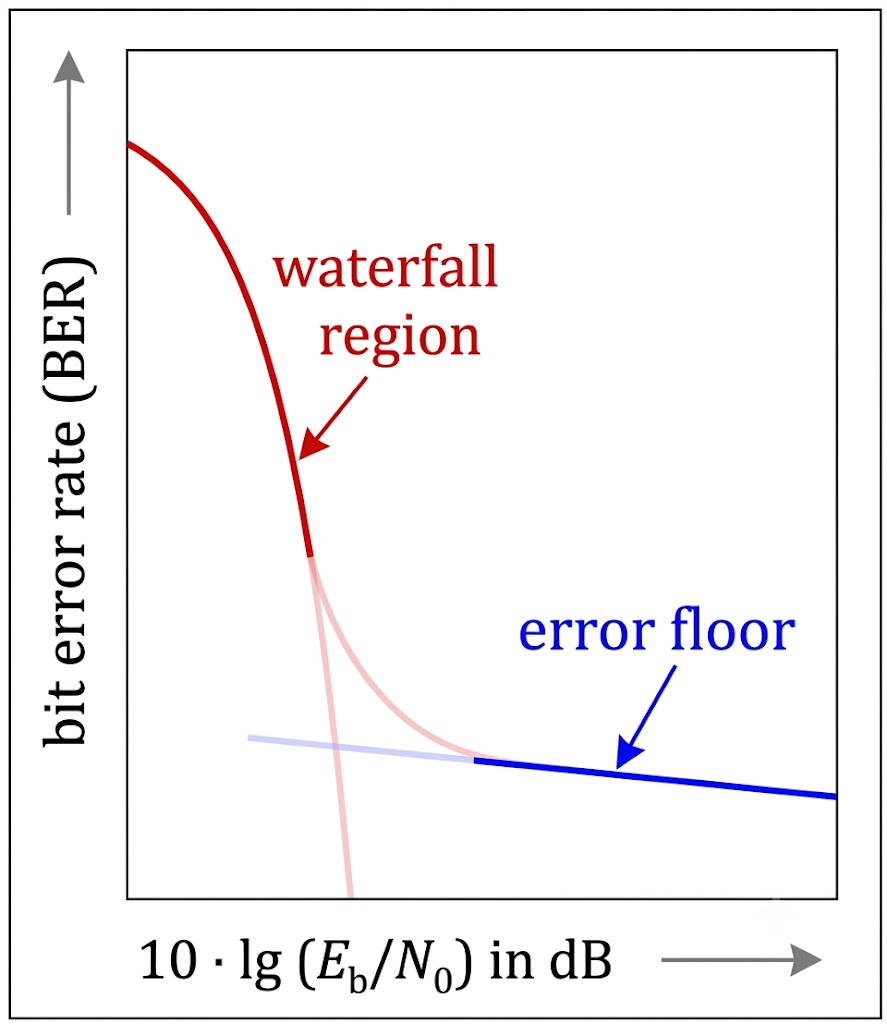
\includegraphics[width=0.5\linewidth]{images/LDPCBehaviour.jpeg}
  \caption{}
  \label{fig: LDPCBehaviour}
\end{figure}

The study of the waterfall region, i.e. over which channel SNR will the BER presents a thresholding effect, is done by density-evolution algorithm. The study of error floor, i.e. what is the BER level of the floor region, is done with the use of combinatorics. However, the reason causing this non-zero floor region can be explained by the trapping sets: at high SNR, the only remaining errors are essentially those where noise happened to land badly on a trapping set.

\textbf{Trapping sets} are defined with respect to the SPA decoder on soft-input channels (e.g. AWGN). A set $\mathcal{T}$ of $a$ variable nodes is an \textbf{$(a,b)$ trapping set} if the subgraph induced by $\mathcal{T}$ has exactly $b$ neighbouring check nodes of odd degree. The decoder gets stuck on $\mathcal{T}$ because only $b$ unsatisfied parity checks signal an error, which is insufficient for the SPA to correct the $a$ erroneous bits. Trapping sets are a decoder-dependent phenomenon --- ML decoding can still succeed where SPA fails.
\begin{figure}[H]
  \centering
  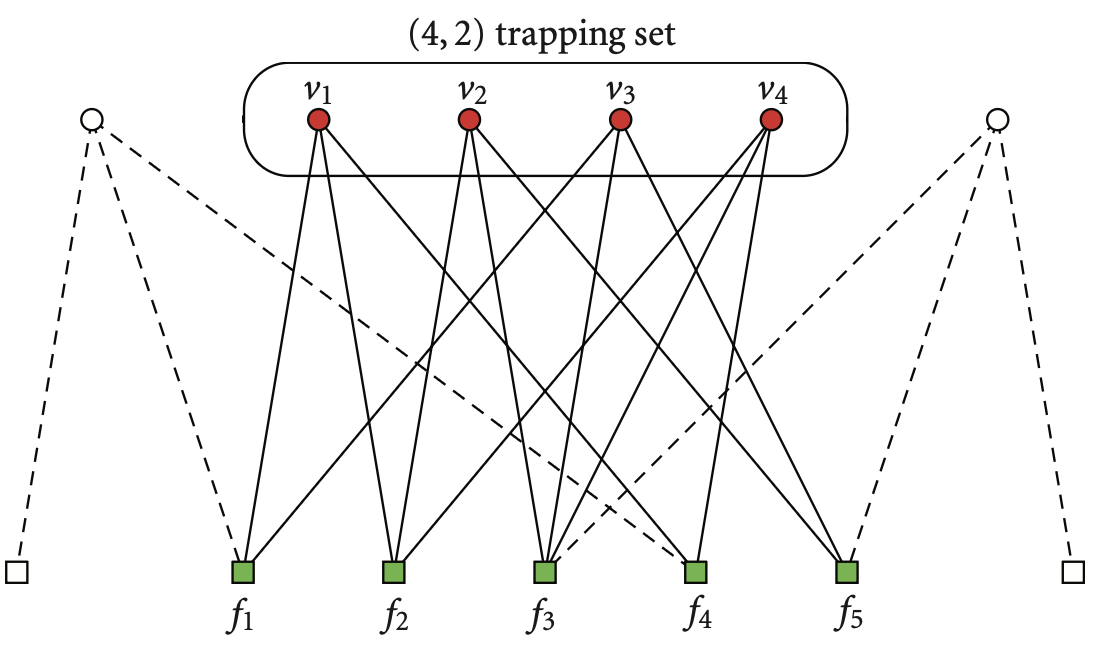
\includegraphics[width=0.5\linewidth]{images/42trappingset.png}
  \caption{Example of a (4, 2) trapping set. Even-degree check nodes are connected to an even number of variable nodes within $\mathcal{T}$, and their LLR update equations are symmetric with respect to the incorrect solution --- wrong incoming LLRs combine to produce outgoing messages consistent with the error, forming self-reinforcing cycles within $\mathcal{T}$ that create a \textbf{stable fixed point at an incorrect solution}. VNs outside $\mathcal{T}$ connected with odd-degree check nodes let them produce corrective messages pushing toward the correct solution, but with only $b$ such nodes against $a$ erroneous variable nodes, their signals are overwhelmed by the stronger reinforcing messages from the even-degree CN cycles.}
\end{figure}

Trapping sets are determined by the Tanner graph structure of $\mathbf{H}$, and contribute to the \textbf{error floor} at high SNR (or low erasure probability). On the BEC, trapping sets and stopping sets coincide --- a trapping set on the BEC is exactly a stopping set, since the only messages are erasures ($L = 0$) or certain ($L = \pm\infty$), and the SPA reduces to iterative erasure filling.



\clearpage
\subsection{Density Evolution}
Iterative decoding of long LDPC codes displays a threshold effect in which communication is reliable beyond this threshold and unreliable below it, in which the threshold is a function of code ensemble properties. 

The main results for iterative decoding of long LDPC codes:
\begin{itemize}
  \item For long LDPC code, this average performance is computable via density evolution. Density evolution refers to the evolution of the probability density functions (pdfs) of the messages being passed around in the iterative decoder, where the messages are modeled as random variables (r.v.s). Thus, we can predict under which channel conditions (e.g., SNRs) the decoder bit error probability will converge to zero. (study of waterfall region in figure \ref{fig: LDPCBehaviour})
  \item \textbf{Concentration theorem} asserts that almost every parity-check matrix $\mathbf{H}$ drawn from the ensemble $\mathcal{C}(n, \lambda, \rho)$ produces a code with similar iterative decoding behaviour (given $n \to \infty$ and fixed $\rho$, $\lambda$), so that the performance prediction of a specific (long) code is possible via the \textbf{ensemble average performance}. The bit error probability of a randomly drawn code concentrates tightly around the ensemble average, with deviations decaying exponentially in $n$. 
  \item For a randomly chosen LDPC code from a given ensemble $\mathcal{C}(n, d_v, d_c)$, and for a fixed number of iterations $\ell$, the neighborhood of depth $2\ell$ around any given edge in the Tanner graph is a tree with probability approaching 1 as the block length $n \to \infty$ (i.e. the codes have a \textbf{cycle-free behaviour}). Density evolution's core computational trick is to use convolution to combine incoming messages, which is only valid if those messages are statistically independent.
  \begin{figure}[H]
  \centering
  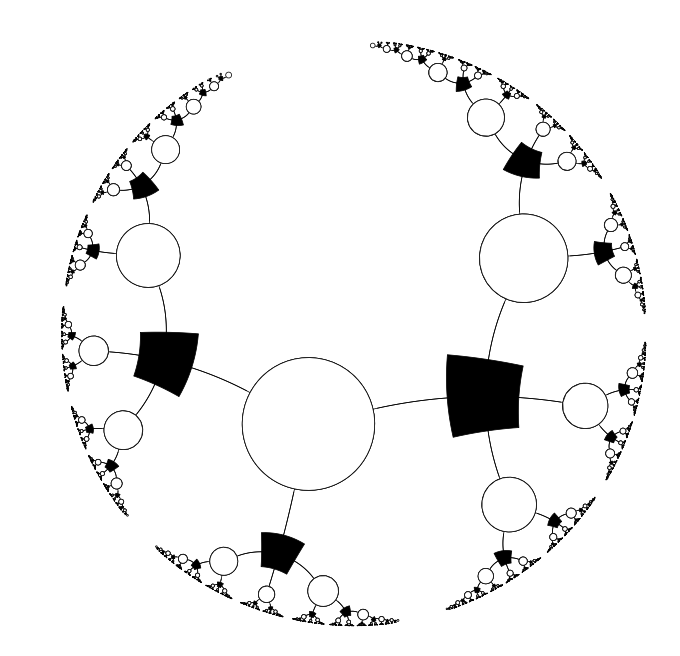
\includegraphics[width=0.4\linewidth]{images/treeLDPC.png}
  \caption{Local topology of the graph of a regular (3,4)-LDPC code. White nodes represent VNs; black nodes represent CNs; each edge corresponds to a 1 in \textbf{H}.}
  \end{figure}
  \item \textbf{Channel symmetry} is also assumed, then we can only compute/track just one message density $p_0^{(c)}$ (assuming the all-zero codeword was transmitted) and have it validly represent decoding performance regardless of which actual codeword was sent. Without symmetry, the error probability depends on which codeword was transmitted.
\end{itemize}

\subsubsection{General Idea}
The computation, via density evolution, of the decoding thresholds for long, $(d_v,d_c)$-regular LDPC code is general, and applies to a number of binary-input, symmetric-output channel models, although we focus primarily on the binary-input AWGN channel. The symmetric-output channel description for the binary-input AWGN channel means that the channel transition pdf satisfies $p(y|x=+1)=p(-y|x=-1)$. It will be assumed throughout that the all-zeros codeword $\mathbf{c}=[0\quad 0\quad \cdots\quad 0]$ is sent. Under the mapping $x=(-1)^c$, this means that the all-ones word $\mathbf{x}=[+1\quad +1\quad \cdots\quad +1]$ is transmitted on the channel.

Because $\mathbf{x}=[+1\quad +1\quad \cdots\quad +1]$ is transmitted, an error will be made at the decoder after the maximum number of iterations if any of the signs of the cumulative variable-node LLRs, $L_j^{\text{total}}$, are negative. Let \textit{$p_{\ell}^{(v)}$ denote the pdf of a message $L_{j \to i}$ to be passed from VN $v$ to some check node during the $\ell$th iteration}. Note that, under the above symmetry conditions for channel and decoder, the pdfs are identical for all such outgoing VN messages. Then, no decision error will occur after an infinite number of iterations if
\[
\lim_{\ell \to \infty} \int_{-\infty}^{0} p_{\ell}^{(v)}(\tau)\,d\tau = 0,
\]
Note that $p_{\ell}^{(v)}(\tau)$ depends on the channel parameter, which we denote by $\alpha$. For example, $\alpha$ is the crossover probability $\epsilon$ for the BSC and the standard deviation $\sigma$ of the channel noise for the AWGN channel. Then the decoding threshold $\alpha^*$ is given by
\[
\alpha^* = \sup\left\{\alpha : \lim_{\ell \to \infty} \int_{-\infty}^{0} p_{\ell}^{(v)}(\tau)\,d\tau = 0\right\}.
\]
If $\alpha > \alpha^*$ then Pr(error) will be bounded away from zero; otherwise, from the definition of $\alpha^*$, when $\alpha < \alpha^*$, Pr(error) $\to 0$ as $\ell \to 0$.

\subsubsection{Density Evolution for Regular LDPC Codes in the BEC}

On the BEC, LLRs take only three values $\{-\infty, 0, +\infty\}$, where $0$ represents an erasure and $\pm\infty$ represents a known bit. Since messages are either erased or known with certainty, the full LLR pdf collapses to a single scalar --- the \textbf{probability of erasure} $p$ along each edge. Tracking the evolution of a full pdf reduces to tracking the evolution of this single probability along the tree structure LDPC code.

For a regular $(d_v, d_c)$ LDPC code on a BEC with erasure probability $\epsilon$, the density evolution update equations per iteration are:
\[
q = 1 - (1 - p)^{d_c - 1} 
\]
\[
p = \epsilon \cdot q^{d_v - 1}
\]
where $q$ is the probability that a check-to-variable message is an erasure, and $p$ is the probability that a variable-to-check message is an erasure. The first equation reflects that a check node can resolve an erasure only if none of its other $d_c - 1$ incoming messages are erased. The second equation reflects that a variable node passes an erasure only if its channel output is erased and all other $d_v - 1$ incoming check messages are also erasures.

Starting from $p^{(0)} = \epsilon$,  
\[
p^{(0)} = \epsilon
\to
q^{(0)} = 1 - (1 - p^{(0)})^{d_c - 1} 
\to
p^{(1)} = \epsilon \cdot (q^{(0)})^{d_v - 1}
\]
\[
\dots
\]
\[
q^{(l)} = 1 - (1 - p^{(l)})^{d_c - 1}
\]
these equations are iterated until convergence. Decoding succeeds if and only if $p^{(\ell)} \to 0$ as $\ell \to \infty$. The \textbf{decoding threshold} $\epsilon^*$ is the largest erasure probability for which this convergence holds, and can be found by analysing the fixed points of the recursion.


\subsubsection{Density Evolution for Regular LDPC Codes}

$m^{(v)}$ denotes the LLRs $L_{j\to i}$, $m^{(c)}$ denotes $L_{i \to j}$ to simplify the notation.
\par\medskip
\par\medskip
\noindent \textit{Variable node update}

To compute $p_{\ell}^{(v)}$, recall that an outgoing message from VN $v$ may be written as
\[
m^{(v)} = m_0 + \sum_{j=1}^{d_v-1} m_j^{(c)} = \sum_{j=0}^{d_v-1} m_j^{(c)},
\]
where $m_0 = m_0^{(c)}$ is the message from the channel and $m_1^{(c)},\ldots,m_{d_v-1}^{(c)}$ are the messages received from the $d_v-1$ neighboring CNs. Now let $p_j^{(c)}$ denote the pdfs for the $d_v$ incoming messages $m_0^{(c)},\ldots,m_{d_v-1}^{(c)}$. Then, with the iteration-count parameter $\ell$,
\[
p^{(v)}_{\ell}
= p_0^{(c)} * \left[p^{(c)}_{\ell - 1}\right]^{*(d_v-1)}
\]
where independence among the messages is assumed and $*$ denotes convolution. The pdfs $p_j^{(c)}$ are identical because the code ensemble is regular, thus, write $p^{(c)}$ for this common pdf. 

\par\medskip
\par\medskip
\noindent \textit{Check node update}

Check nodes combine rule in the sum-product algorithm is not a simple sum in the LLR domain, it follows the $\tanh$ rule:
\[
\tanh(\frac{1}{2} m^{(c)}) = \prod_{v = 0}^{d_c - 1} \tanh\left(\frac{1}{2}m^{(v)}\right),
\]
Since density evolution needs convolution to combine independent random variables efficiently, we need to first transform messages into a domain where the check-node combining rule becomes additive instead of multiplicative. So, let $\Gamma$ be a function transforms the variable-to-check message density $p^{(v)}_{\ell}$ into a domain where the check-node rule becomes additive and its inverse $\Gamma^{-1}$ is the transformation back to the usable LLR domain. Then,
\[
p_\ell^{(c)} = \Gamma^{-1}\left[\left(\Gamma\left[p_\ell^{(v)}\right]\right)^{*(d_c - 1)}\right]
\]


\begin{algorithm}[H]
\caption{Density Evolution for Regular LDPC Codes}
\begin{algorithmic}[1]
\State Set the channel parameter $\alpha$ to some nominal value expected to be less than the threshold $\alpha^*$. Set the iteration counter to $\ell=0$.
\State Initialize $p_0^{(c)}$ which is the probaility density of initial channel LLR, $m_0 = \log\left( \frac{\text{Pr}(y_i \mid x_i = 0)}{\text{Pr}(y_i \mid x_i = 1)} \right)$, from the channel property. Given $p_0^{(c)}$, obtain $p^{(v)}$ via the VN update equation, with $m^{(c)}=0$ initially.
\State Increment $\ell$ by $1$. Given $p^{(v)}$, obtain $p^{(c)}$ using CN update equation.
\State Given $p^{(c)}$ and $p_0^{(c)}$, obtain $p^{(v)}$ using the VN update equation.
\State If $\ell < \ell_{\max}$ and
\[
\int_{-\infty}^{0} p^{(v)}(\tau)\,d\tau \leq p_e,
\]
(assuming the all-zero codeword / positive-LLR-correct convention)
for some prescribed error probability $p_e$ (e.g., $p_e=10^{-6}$), increment the channel parameter $\alpha$ by some small amount and go to Step 2. If the inequality does not hold and $\ell<\ell_{\max}$, then go back to Step 3. If the inequality does not hold and $\ell=\ell_{\max}$, then the previous $\alpha$ is the decoding threshold $\alpha^*$.
\end{algorithmic}
\end{algorithm}



\end{document}